%\newpage
\section{Experiments}
\label{sec:experiments}
\subsection{Dataset and Experimental Setting}
\subsubsection{Dataset}
\label{subsec:Dataset}
In our research center, we maintain a big transportation data warehouse that fuses and analyzes a very large-scale and high-resolution (both spatial and temporal) traffic sensor data from different transportation authorities.  This data set includes both historical and real-time data with update
rate as high as every 30 seconds for freeway and arterial traffic sensors (9300 loop-detectors) covering more than 3500 miles, incidents  such as accidents, traffic hazards and road closures reported (approximately 400 per day), and ramp meters. 
We have been continuously collecting and archiving aforementioned datasets for the past three years. We use this real-world dataset to model and evaluate our techniques. To generate time dependent  travel times we spatially and temporally aggregate traffic sensor data by assigning interpolation points for each 5 minutes during a year that
depict the travel-times on the segments of a major metropolitan road network with 304,162
edges. Based on our observation, all roads are fairly un-congested between 9:00pm and 6:00am, and hence we assume static edge weights between those times.

\subsubsection{Experimental Setting}
All experiments were conducted on an Intel(R) Core(TM)2 Duo 3.16GHz PC running on Microsoft Windows 7. Methods were implemented in Java.

Predicting travel times in a rather static road network (with only marginal
changes in the link travel times) is obviously not very challenging and usually does not require a probabilistic prediction. For this reason we focused on rush hour times which imply a lot of traffic and thus a much harder scenario for prediction. Specifically, if not mentioned otherwise we used 8:00am, 9:00am, 4:00pm, 5:00pm and 6:00pm during the week. These times were considered as the \textit{start time}, i.e. the time at which the user starts his route.
According to the results from \cite{Pan12} and our own observations, traffic patterns are quite equivalent across weekdays. Consequently, we did not differentiate between predictions for different weekdays. Thus for each start time we consider data of 260 days (5 days per week, 52 week per year). In our evaluation process, we used the k-fold cross validation (k=5) method to divide our data into test (test days) and training (training days) sets. In each fold, for each start time and each test day we investigated the following:
\begin{itemize}
  \item The true certain result. In the case of a link travel time, this
  value can be looked up in the data. In the case of the path travel time, this
  value can be straightforwardly computed by taking into account the changing values
  of link travel times during the completion of the route.
  \item The probabilistic prediction based on the readings of the training days
  (and possibly the current situation), using the techniques proposed in Section
  \ref{sec:lttestimation} (for link travel times) and Section \ref{sec:methods}
  (for path travel times).
\end{itemize}
Both of these outcomes are then used to compute a CRPS score as defined
in Section \ref{sec:evaluate}, which is then averaged over all folds and trials.
For all discrete models we discretized the time into 1 second intervals.

\subsection{Probabilistic Link Travel Time Prediction}
In our first set of experiments we evaluate the prediction quality of
the following three proposed approaches:
\begin{itemize}
  \item HP: Prediction purely based on historical data as described in Section
  \ref{subsec:historical}.
  \item LI: Prediction based on linear interpolation between the current
  situation and the prediction based on historical data as discussed in Section
  \ref{subsec:LI}.
  \item SH: Prediction based on historical data with similar behaviour than the
  current situation as proposed in Section \ref{subsec:SH}.
\end{itemize}

We tested all approaches for 50 edges which are chosen randomly from all around the road network explained in \ref{subsec:Dataset}. 

The farther an event is in the future, the harder it gets to predict it. Therefore we introduce two concepts in addition to \textit{start time}, to demonstrate how far in the future we want to make a prediction for. The time at which a user makes a query to predict something in the future is called
\textit{query time} and \textit{start time} will be the time at which the user wants the prediction for. The difference between these two times is called \textit{prediction offset}. For example, at time 7:45am (\textit{query time}) a user makes a query to predict the link travel time at 8:00am (\textit{start time}). Here the \textit{prediction offset} will be 15 minutes. In our experiments we consider \textit{prediction offsets} from 5 minutes up to 120 minutes.

% We assume that Mondays, Tuesdays, Wednesdays and Thursdays have similar
% traffic patterns. We run our tests for different start times during these four
% days. We consider 5 different base start times during a day: 8:00, 11:00,
% 14:00, 17:00 and 20:00.

% In our evaluation process, we use the K-fold cross validation method to decide
% which days to use to build the model and which days to do the tests. Overall
% for each start times we have $\sim$200 target days to consider; 4 days per
% week, 52 week per year. In the experiments we choose k = 5, meaning that we
% divide our target days into 5 equally sized sets. Each time we use one set as
% the test data (test days) and the remaining sets as model data (model days).
% We build the model distribution using the readings at a specific time in the
% model days. Then for each data item in the test set, we compute the actual
% travel time for the start time in the test day and compare it with the model
% distribution. We check the accuracy of the prediction using the \emph{CRPS}
% method defined in section \ref{sec:evaluate}.
% For each representation and each start time during the day, we take the
% average score given by the \emph{CRPS} method and compare the results for
% different start times and both continuous and discrete link travel time
% representations.\\

\begin{figure}[h]
	\centering
	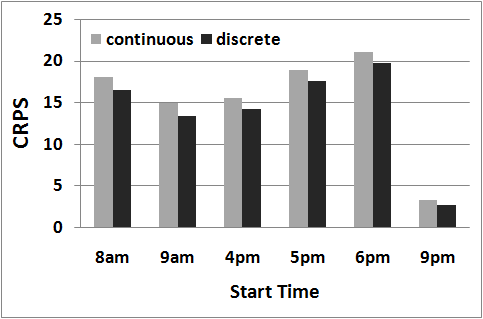
\includegraphics[width = 0.65\columnwidth]{figures/HP_results.png}
			\vspace{-0.2cm}
	\caption{CRPS Score for HP Approach}\label{fig:HP_results}
			\vspace{-0.2cm}
\end{figure}

With the HP approach, we only consider historic data. This means that if we use 8:00am as the \textit{start time}, we consider the travel times at 8:00am across the training days and build the model distribution. Subsequently, we retrieve the actual travel time at 8:00am for each test day and compare it with the model. Since the historic approach is based on historical data only and does not incorporate knowledge about the current situation (\textit{query time}), it is consequently independent form the \textit{prediction offset}. The results for the HP approach are shown in Figure \ref{fig:HP_results} and show two implications. First, different times of the day are differently hard to predict. In particular the selected standard start times yield much higher CRPS compared to 9:00pm, where there is not too much traffic on the road network and thus not a lot of uncertainty in the prediction.  Second, it shows that the continuous and discrete representation performs rather equivalent. The small difference between the discrete and the continuous case can be explained by the fact that a discrete representation copes better with non-normally distributed link travel times. However, it is important to note that the CRPS of the discrete representation is very sensitive to the discretization interval of the time, i.e., a large discretization interval leads to a larger value of the CRPS and hence not directly comparable to the CRPS of the continuous representation.
Since the results for continuous and discrete link travel times are rather
equivalent across all experiments regarding link travel time prediction, we focus only on the discrete case in the rest of this subsection.


\begin{figure}[h]
    \centering
    \subfigure[Different time horizons]{
        \label{fig:LI1}
        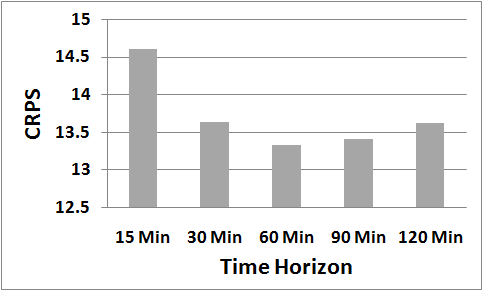
\includegraphics[width = 0.7\columnwidth]{figures/LI1_results.png}
    }
    \subfigure[Different values of $\theta$]{
        \label{fig:LI2}
        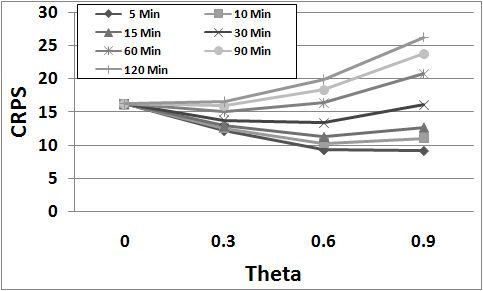
\includegraphics[width = 0.7\columnwidth]{figures/LI2_results.png}
    }
        		\vspace{-0.2cm}
    \caption{Experiments for the LI approach}\label{fig:LI_results}
    		\vspace{-0.4cm}
\end{figure}



With regards to the LI approach, we studied the accuracy of the model for
different time horizons $\tau$, ranging from 15 minutes up to 120 minutes. Using a small time horizon $\tau$ is basically favoring the historic data, whereas setting $\tau$ to a large value weights the current situation higher. The results in Figure \ref{fig:LI1} are averaged over all \textit{prediction
offsets} and clearly show neither of these extremes should be chosen, but rather a good choice of the time horizon is somewhere in between (i.e., around 60 minutes). These results are backed up by the experiments shown in Figure \ref{fig:LI2}. In the LI approach, we eventually use the time horizon to compute $\theta$ as the weight of the current situation versus historic data. In Figure \ref{fig:LI2} we directly assign different values to $\theta$. If increasing $\theta$ yields better results, it means assigning more weight to the current situation is beneficial and vice versa. Figure \ref{fig:LI2} shows that for prediction offsets greater or equal to 60 minutes, increasing $\theta$ does not give better CRPS scores. Hence we can say, the current situation has no positive influence on the prediction after 60 minutes, which is the definition of the time horizon parameter in Section \ref{subsec:LI}.


\begin{figure}[h]
	\centering
	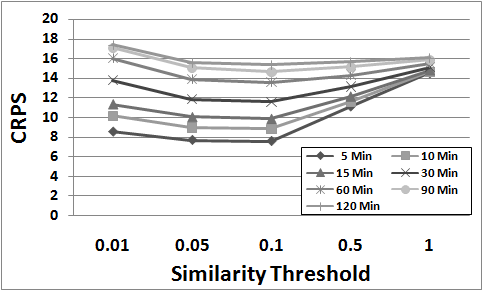
\includegraphics[width = 0.7\columnwidth]{figures/SH_results.png}
	\caption{CRPS Score for SH Approach}\label{fig:SH_results}
\end{figure}

In the next set of experiments, we evaluate the accuracy of the SH approach. As
explained in Section \ref{subsec:SH}, SH only considers the historical data
similar to the current situation. For example, for \textit{query time} 7:45am on
Jan 1st, 2013, and predicting 15 minutes in the future (\textit{prediction
offset}), we only consider the travel times at 8:00am for those days in the model
days, were the travel time  at 7:45am is similar to Jan 1st, 2013.
Similarity is defined by the parameter $\lambda$ representing the percentage
by which a travel time may maximally differ in order to be accepted as similar. 
We assign different values to $\lambda$ and compare the results. Figure
\ref{fig:SH_results} shows the results. Like LI, SH predicts the near future
more accurate than the far future since it is taking the current situation into
account. For smaller values of $\lambda$ (e.g., 0.01 \& 0.05), however, the
predictions yield generally higher CRPS. The reason for this behavior is
that only very few measurements of the training data meet the similarity
requirement and thus the prediction is based on a possibly non-representative
sample. Therefore, as the similarity threshold increases, our model gets more
realistic and the results get better. On the other hand, if the similarity
threshold is too loose, data that is not similar to the test day is
considered in generating the model, which results in less accurate models.
Eventually at $\lambda = 1$ the prediction model converges to the historical
approach.

\begin{figure}[h]
	\centering
	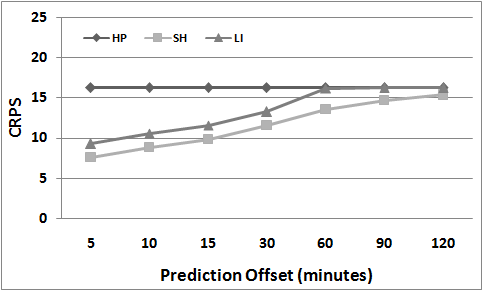
\includegraphics[width = 0.7\columnwidth]{figures/link_results.png}
	\caption{CRPS Scores for HP, LI and SH}\label{fig:all_results}
\end{figure}

Finally, we compared the three approaches to each other, using the best setting
for the corresponding parameters ($\tau = 60$ minutes and $\lambda = 0.1$). The
results are illustrated in Figure \ref{fig:all_results}. Clearly, LI and SH are
able to predict the near future more accurately than the farther future, whereas
HP is independent from the \textit{prediction offset}. Resulting from the
setting of the time horizon, LI converges to HP at 60 minutes, whereas SH
converges at 2 hours. It seems that behind this temporal ``barrier'', the
current situation does not help in predicting the future on a road network anymore.
Overall SH yields the best performance of all approaches and we will primarily
use this method to evaluate the approaches computing the path travel
time.

